\documentclass[12pt,letter]{article}
\usepackage[margin=1in]{geometry}
\usepackage{lineno} %line numbering
\usepackage[round]{natbib} %bibliography
\usepackage[english]{babel}
\renewcommand{\baselinestretch}{1} %adjusts line spacing (currently set to single-space)
\usepackage{graphicx} %import figures
%\usepackage[nomarkers, tablesfirst]{endfloat} %for placing figures
\usepackage{amsmath} %some math symbols
\usepackage{rotating} %rotate table 90-degrees
\usepackage{color, xcolor} %make text colors other than black
\usepackage{setspace}
\usepackage{subcaption} %subcaptions for subfigures


\definecolor{mypink1}{rgb}{0.75, 0, 0.75}

% commands for notes from Katie
\newcommand{\kpd}[1]{\textcolor{mypink1}{[Katie: #1]}}
\newcommand{\mnpv}[1]{\textcolor{blue}{#1}}
\newcommand{\snpv}[1]{\textcolor{red}{#1}}
\newcommand{\addref}[1]{\textcolor{blue}{(ref#1)}}



\title{Automating data analysis of weather information related to Douglas Fir Tussock Moth Projects}
\date{March 22, 2019}
\author{Katherine Dixon}

\begin{document}
\raggedright
\setlength{\parindent}{25pt}
%\linenumbers

%\tableofcontents
%\listoffigures 
%\listoftables



\maketitle
%-----------------------------------------------------------------------------------------%
%					INTRODUCTION					%
%-----------------------------------------------------------------------------------------%

\subsection*{Questions addressed}

The Dwyer lab has a project working with the USDA Forest Service trying to manage Douglas Fir Tussock Moth (DFTM) populations by trying to predict population dynamics. The dynamics we focus on are how much the caterpillars are going to eat (defoliation) and whether or not natural virus in the population will effectively control the population. If the local DFTM populations are high enough, but not so high that it crosses a disease threshold, the Forest Service will spray virus in the area, which is very costly. The projects in the lab are all management related, to varying degrees, and are focusing on different aspects of the system. 

While we are always focused on the biology and phenology of the virus and the tussock moth caterpillars, it is very intertwined with site specific differences in weather, altitude, latitude, and tree species composition. These populations range from New Mexico and Arizona, up the Rocky Mountains through Colorado and California, to British Columbia and Canada. Questions we are constantly asking ourselves are 1) when does the snowpack melt so we can go collect feral eggs to use in our experiments, 2) around what times do bud burst on the trees and egg hatch occur so that we can time our experiments and 3) what are the weather related site specific differences that might explain some of the different patterns we see in the tussock moth populations. 

These questions come up constantly. To answer questions about when snowpack melts, our usual method is to go look up the NOAA Interactive Snow Information website, which visualized snowpack for a given area, and put in GPS coordinates and random dates until we can see a date with no snow in the past. While I think this is nice for visualizing our sites, it is time intensive and doesn't give us that much information, we also then never write any of this information down, so we have to do this repeatedly. 

To answer questions about tree and caterpillar phenology for each site, we usually have to ask the Forest Service if anyone has any data on when the caterpillars emerged in previous years in those locations. Often, there is not much information or it is based on anecdotal evidence. This is relevant to my experiments because I want to be able to time when I put the caterpillars out on covered branches for my experiment to when that instar of caterpillar would actually be there in natural populations. This question has recently been coming up for Will Koval's experiment for the summer of 2019 because he wants to track the dispersal movements for first instar caterpillars, so he needs to be in the right location at the right time. While this is always a lot to ask for, since there is a lot of stochasticity in weather patterns, it would be nice to have a plan.  

We would also like to be able to see if there is a difference between sites in temperature, weather, or the timing of events like snow pack. This would answer questions about years or sites that don't fit our models based on previous data and would help the Forest Service plan. 

\subsection*{Methods for answering questions}

I was hoping I would be able to find a way to quickly download temperature and weather datasets through NOAA for sites I was interested in. However, I had to download the datasets manually through the NOAA Climate Data Online: Dataset Discovery webpage. This involves finding the right weather station with good amounts of data near our field sites, putting in the dates, clicking on what type of data you want, making sure you ask for a CSV file and not a PDF, and then check out from your shopping cart and wait a minute for NOAA NCEI to email it to you. The downsides of this is that it takes a lot of clicks to actually get the datasets and you can only do one at a time because there are limits to the amount of 'station years' you can download at one time. The upsides are that you only have to do it once and then you have the dataset forever. 

I downloaded four datasets from some weather stations near our field sites in New Mexico, Idaho, and Washington to test my methods on (Table \ref{table:1}). I have good experience using R for mathematical modeling and statistical analyses, but I have always wanted to become fluent in \textit{tidyverse} and \textit{ggplot}. I had only been exposed to it during MBL bootcamp and hadn't had the opportunity or motivation to use it since. So, I tried using techniques we were introduced to in class and other things I'd seen people do to solve the questions I had. 


\begin{table}[h!]
\centering
\begin{tabular}{l c c c c} 
 \hline
 Site name & Station name & Location & Approx. elevation (ft) & No. years full dataset \\
 \hline
Craters of the Moon & Craters & ID & 4,800 & 59 \\
Sage Hen Reservoir & Emmett & ID & 4,800 & 87 \\
Leavenworth & Leavenworth & WA & 1,171 & 103 \\
Balsam Glade & Sandia & NMX & 8,650 & 67 \\
 \hline
\end{tabular}
\caption{Table of information about field sites and their locations, includes number of years in the full dataset (not the one provided). }
\label{table:1}
\end{table}

Each dataset had daily information on precipitation, temperature, and other things that I was less interested in for up to 105 years. The datasets I provided are limited to only 20 years to limit computing time, I hope that is a small enough dataset. I got rid of all of the information besides precipitation, snowfall, snow depth, temperature maximum, and temperature minimum. I wrote all my functions to manipulate the data in a file called \textit{Functions.R} so that I could load all the functions at once when I needed them. In a separate file called \textit{Data\_testing.R}, I wrote where I look at and clean up some of the data, to get rid of years where there isn't enough days of information and add columns for the months and years. I set a few global parameters dealing with tussock moth biology. I decided not to remove all the \textit{NAs} because for some of the datasets there is a lot of information about TMAX and TMIN and less about things like snow depth, but I wanted to keep that information.

My goal for the functions was to be able to input an upper and lower time bound and in some cases a variable to get a plot with the correct location as the title. I was mostly successful in this! In general, I would begin by subsetting the data in between the years given, define a variable of interest, summarize it over years, and then plot the data using \textit{ggplot}. Here is a list of functions:


\begin{enumerate}
   \item \textit{plot\_over\_time} can choose to plot any variable over time, for each day 
      \begin{enumerate}
     \item e.g. Temperature maximum, 
     \item Temperature maxima example (Figure \ref{fig:LTempMax})
   \end{enumerate}
   \item \textit{TMAX\_over\_time} plots early temperature maxima over time
   \item \textit{TMIN\_over\_time} plots yearly temperature minima over time
   \item \textit{ETREMES\_over\_time} plots yearly temperature extremes over time
   \item \textit{last\_no\_snow} plots last day of the year when there is clear ground (no snow)
   \item \textit{first\_no\_snow} plots day of the year when there is clear ground
        \begin{enumerate}
     	\item Trouble here because sometimes there is clear ground in January
   	\end{enumerate}
   \item \textit{cumulative\_snow} plots cumulative snowfall for the year
   \item \textit{find\_degree\_days} finds number of Julian days to reach some degree day target given a threshold
   \item \textit{degree\_days\_time} finds degree days to reach same target for each year given given a threshold, can choose to plot or not
   \item \textit{plot\_degree\_days} plot either cumulative degree days or how many degree days each day provides 
           \begin{enumerate}
     	\item (Figure \ref{fig:cumulativeDD})
   	\end{enumerate}
 \end{enumerate}


\begin{figure}
\centering
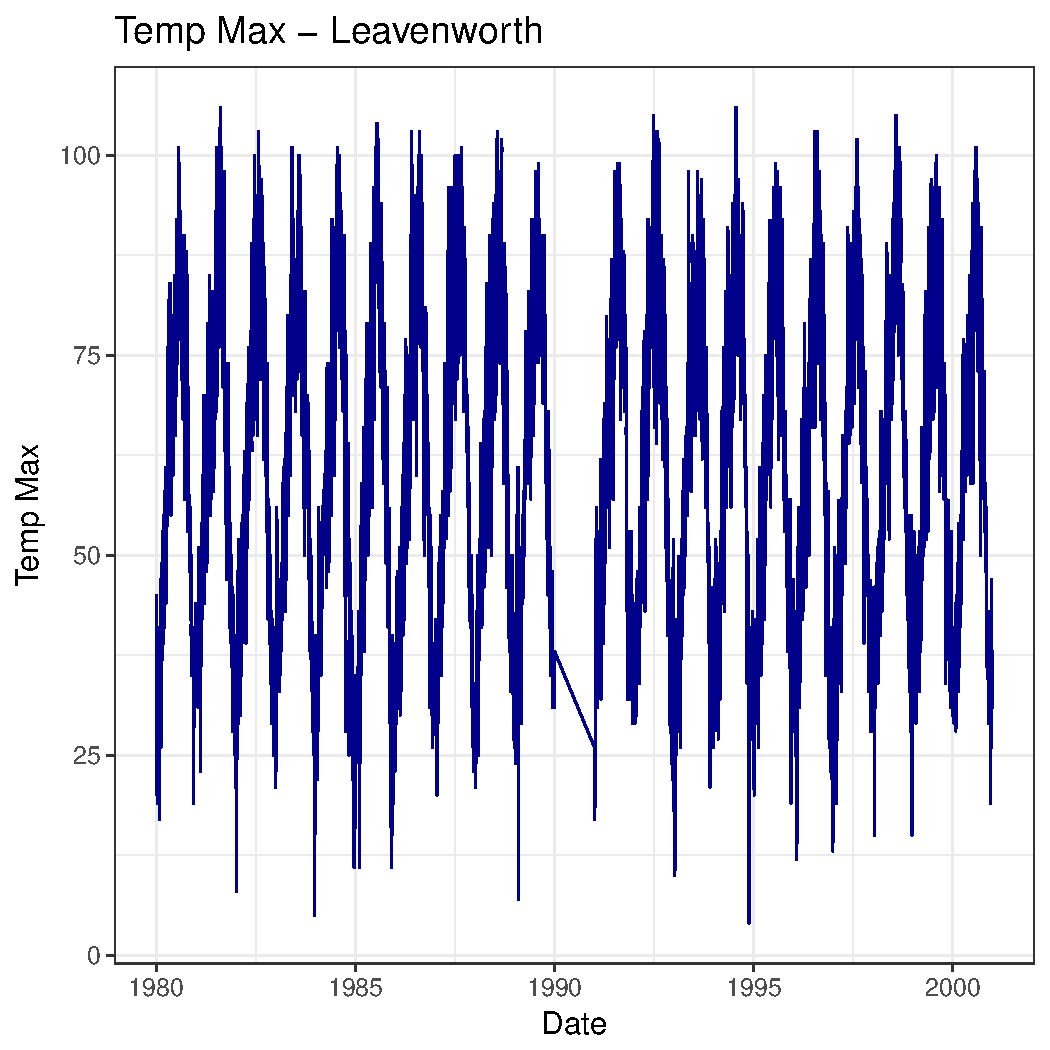
\includegraphics[width = 0.5\textwidth]{../Plots/TMAX_Leavenworth_KD.pdf}
\caption{Daily temperature maximum for Leavenworth, WA over time.}
\label{fig:LTempMax}
\end{figure}


\begin{figure}
\centering
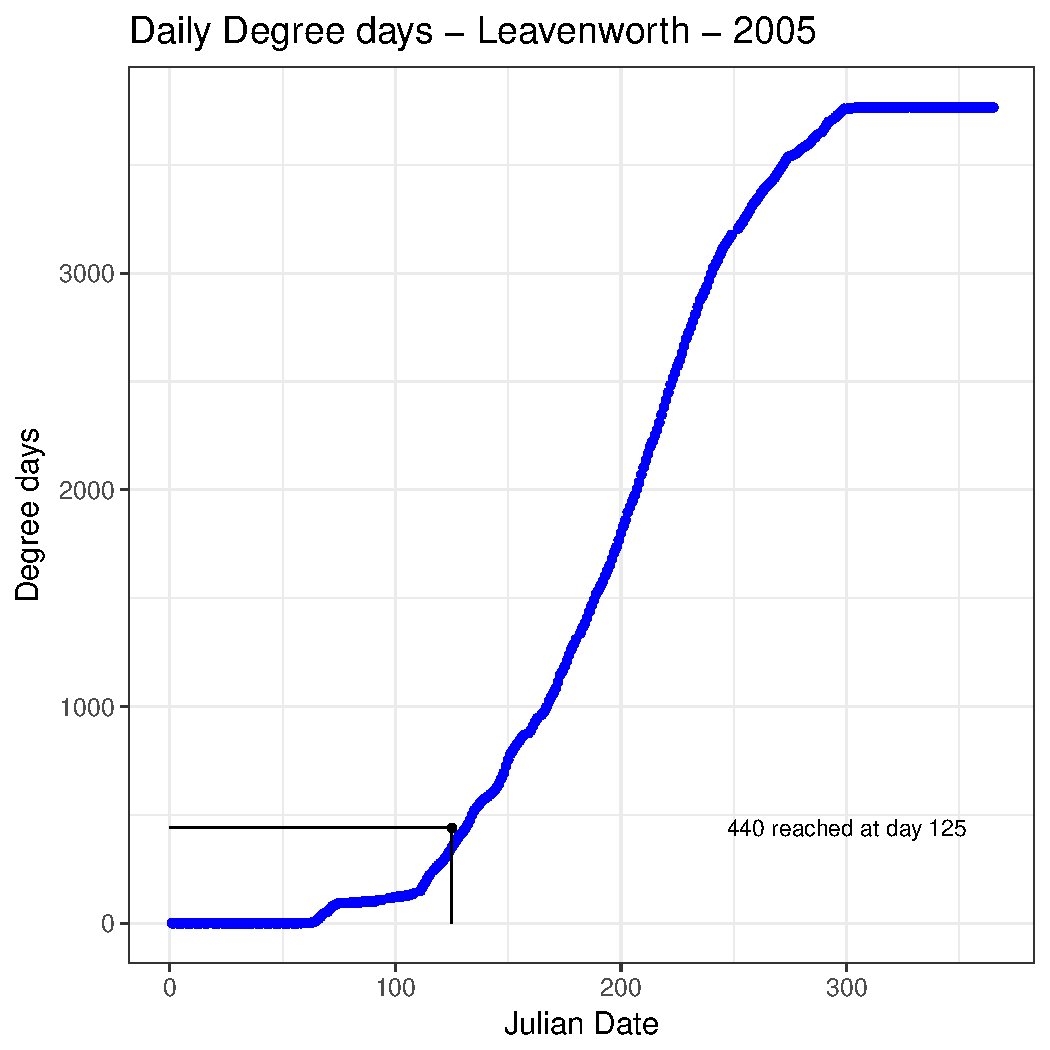
\includegraphics[width = 0.5\textwidth]{../Plots/cumulative_Leavenworth_KD.pdf}
\caption{Daily temperature maximum for Leavenworth, WA over time.}
\label{fig:cumulativeDD}
\end{figure}

For degree days it was more complicated. I had to define some $\text{T}_{\text{DFTM}}$ that was the threshold above which tussock moth caterpillars start developing in their eggs, which is estimated to be 42$^\circ$F. I had to define some target for degree days, which is when the tussock moths have ideally finished developing and will start to hatch, this is estimated to be about 440 degree days. I had to write a function that calculated: 

$$ \frac{\text{TMAX} + \text{TMIN}}{2} - \text{T}_{\text{DFTM}} $$ and then set all the negative values to zero, because tussock moths aren't developing below that threshold. I then had to find the number of Julian days it took to reach that threshold, which would be the estimate for when tussock moths hatch. 

I then had to write a function that looped over the years and calculated the number of Julian days it took to reach that threshold, find the mean, variance, and the plot is optional. 

% bud burst started between 244 and 268 degree-days (F)
% 90 percent of bud burst occurred between 340 and 444 degree days (F)
% the treshold is 42 degrees F in tussock moths

I wanted to write a script that would take all the files in a folder and calculate the mean and variance in number of days it took to reach the 440 degree days, so that I could collect the information for several sites at one time. This script is \textit{Predictions\_2019.R}. To do this I had to define a file directory and create a list of the filenames in the directory. Then I had to load each file in a for loop and run the functions to calculate the mean and standard deviations. I then put the dates back into month and day format, because that's how humans (Will and I) are used to reading it. Now we would be able to see the windows during which we should plan to be out west if we want to catch first hatch (Figure \ref{fig:DDbysite}). Ideally, I could adapt this code do this for other variables, like the estimated day that there is no snow left on the ground in spring.

\begin{figure}
\centering
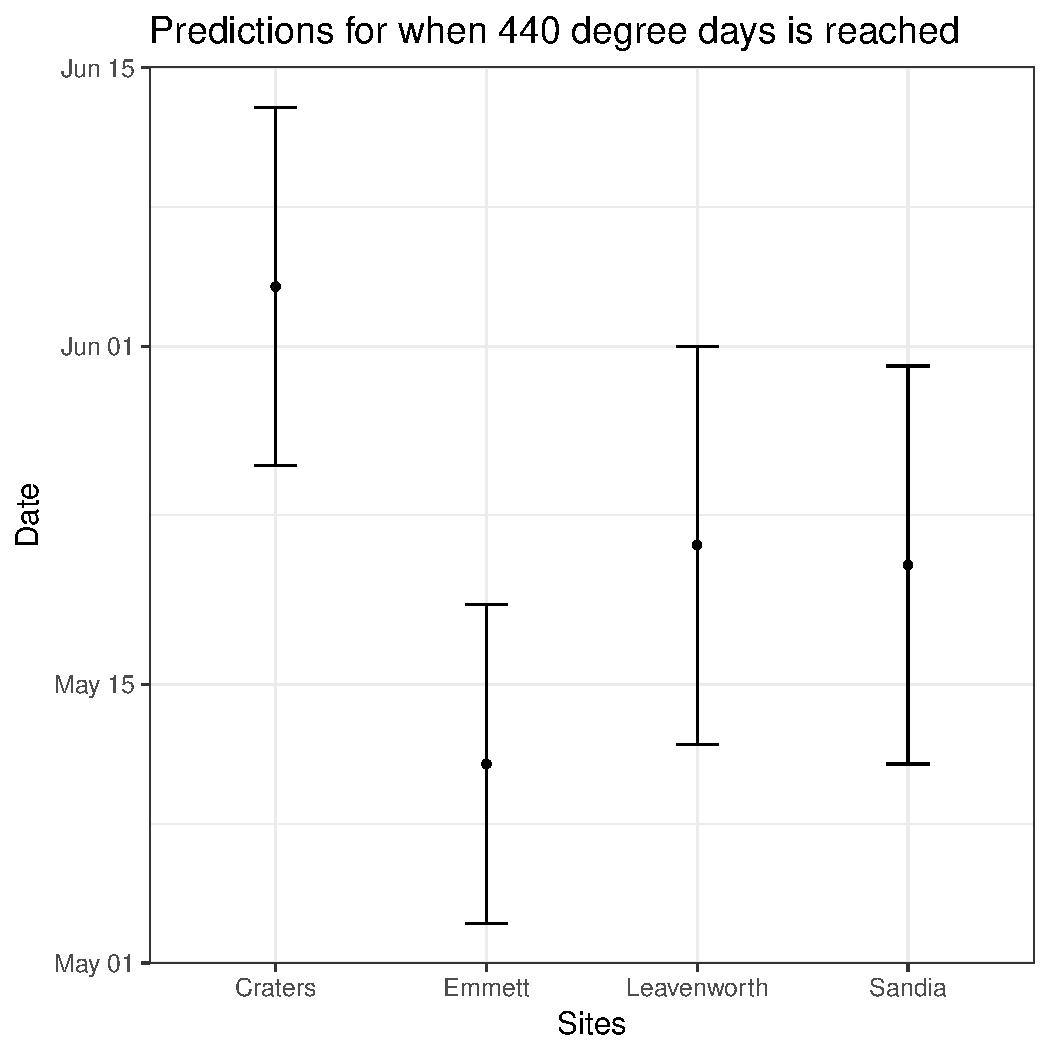
\includegraphics[width = 0.5\textwidth]{../Plots/2019Pred_KD.pdf}
\caption{Daily temperature maximum for Leavenworth, WA over time.}
\label{fig:DDbysite}
\end{figure}

The next steps are to match this with actual emergence data, because there is potentially local adaptation by the DFTM caterpillars, but that is an ongoing project in the Dwyer Lab. This could easily be adapted to look at any insect or tree whose phenology can be estimated by degree days, as long as there is information on the threshold above which development begins and number of days needed to reach that value.



%-----------------------------------------------------------------------------------------%
%				  LITERATURE CITED			       		%
%-----------------------------------------------------------------------------------------%
\pagebreak
%\bibliographystyle{apalike}
%\bibliography{DFTM.bib}


\end{document}